\section{Single axis experiments}
We have been doing the synthesis of controller using different reduction of the second integrator model, we will compare the results to the raw second integrator model.
As we have seen in the previous parts, there is no need to test different values than the $\Delta n_u = 0$ and $\Delta n_u = 1$.
The case $\Delta n_u = 0$ (mode without any memories) correspond to the case of the single integrator.

\comment{Things to explains:
\begin{itemize}
\item How to choose the sampling time
\item How to configure the model
\item Speed profiles (add the velocity commands)
\item Computation of the time
\end{itemize}
}

For each of the models, the solution plans has been generated so that they have the less state as possible.


\subsection{Second integrator model with velocity feedback}
\begin{figure}[!ht]
	\begin{minipage}[b]{0.5\textwidth}
  		\centering
  		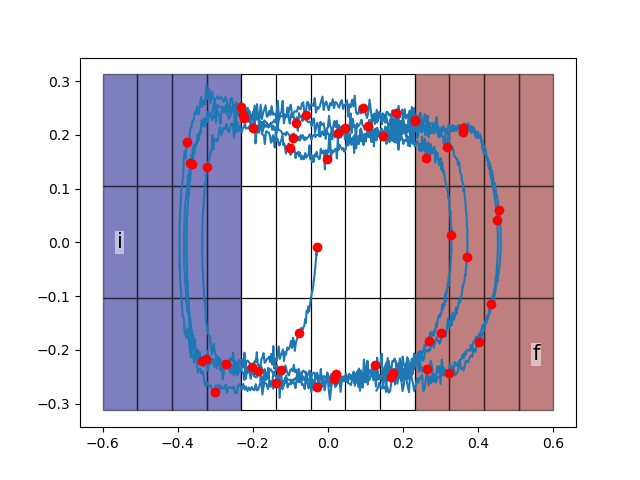
\includegraphics[width=0.9\linewidth]{double_1D}
	  	\caption{Trajectory in the 2D environment.}
	  	\label{double_1D}
  \end{minipage}
	\begin{minipage}[b]{0.5\textwidth}
  		\centering
  		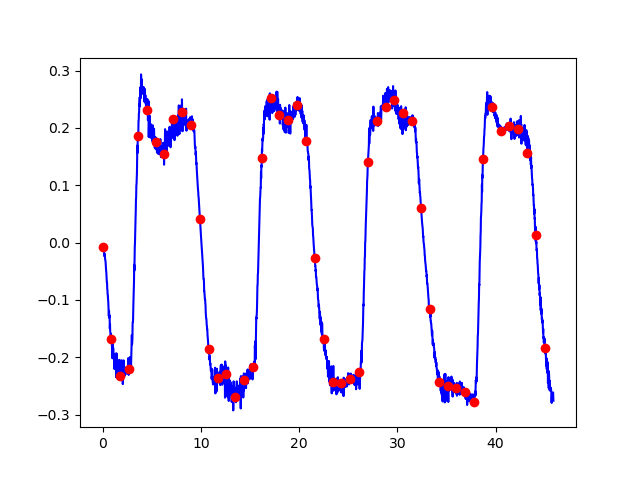
\includegraphics[width=0.9\linewidth]{double_1D_vel}
	  	\caption{Velocity profile.}
	  	\label{double_1D_vel}
  \end{minipage}
  \caption{Trajectory and velocity profile of the double integrator model. The agent is trying to achieve 'go infinity often to i and f'.}
\end{figure}

The model used is the "raw" second integrator model with velocity feedback.

%% SELF LOOPS ON THE VELOCITY AXIS
When creating the abstraction for such a model, the self loops are acceptable only for some controls and cell combinations. 
If the velocity of the quad is positive and the reference velocity negative, any self loop on the velocity axis will "keep" the next velocity state to the same cell.
This will create abstractions that are not controllable.
\comment{Do a graph about it}

\comment{plot the noise}

The second integrator model manage to take in account the transient state that was hidden by the single integrator model: in $x\approx0.4$, the transient states is clearly going "backward", this show that this model is not usable with the single integrator model (which correspond to non reachability behaviours).

\subsection{Model with $\Ninputs= 1$ memory}
\begin{figure}[!ht]
	\begin{minipage}[b]{0.5\textwidth}
  		\centering
  		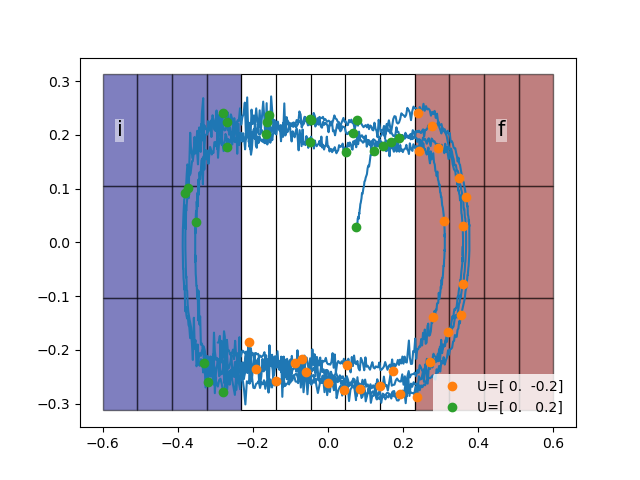
\includegraphics[width=\linewidth]{double_reduced_1D}
	  	\label{double_reduced_1D}
  \end{minipage}
	\begin{minipage}[b]{0.5\textwidth}
  		\centering
  		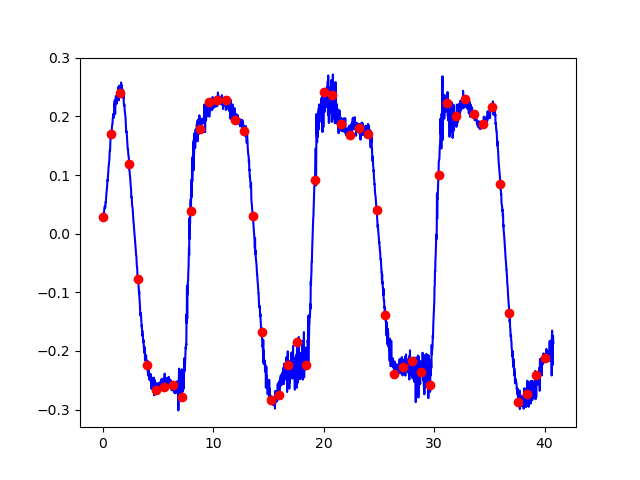
\includegraphics[width=\linewidth]{double_reduced_1D_vel}
	  	\label{double_reduced_1D_vel}
  \end{minipage}
  \caption{Trajectory and velocity profile of the double integrator reduced model. The agent is trying to achieve 'go infinity often to i and f'.}
\end{figure}

In our setup, the sampling time of model is ${\Delta t = 1s}$ and the timing constants of the reduced system is $\tau_r = {\nicefrac{1}{k} = 0.7s}$. This make relevant to use this reduction method as the internal dynamic of the quadricopter are not vanished enough after a $\Delta t$.


\subsection{Model with $\Ninputs= 1$ memory} \label{sec:single_int}
\begin{figure}[!ht]
	\begin{minipage}[b]{0.5\textwidth}
  		\centering
  		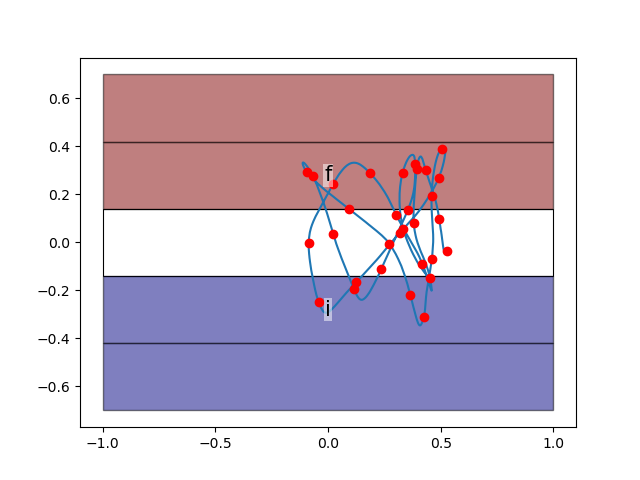
\includegraphics[width=0.9\linewidth]{simple_1D}
	  	\label{simple_1D}
  \end{minipage}
	\begin{minipage}[b]{0.5\textwidth}
  		\centering
  		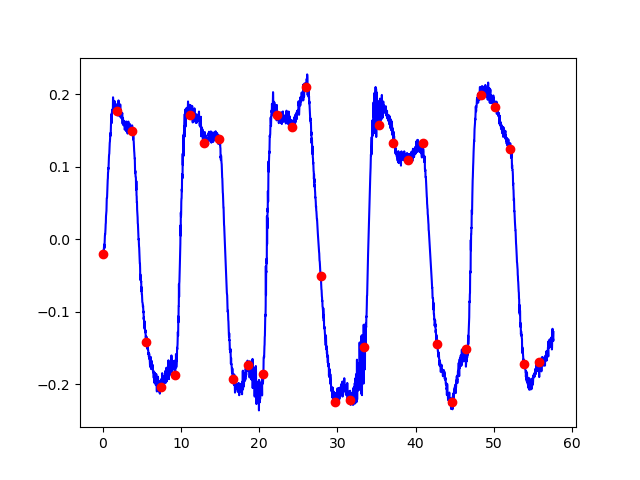
\includegraphics[width=0.9\linewidth]{simple_1D_vel}
	  	\label{simple_1D_vel}
  \end{minipage}
  \caption{Trajectory and velocity profile of the simple integrator model with self loops. The agent is trying to achieve 'go infinity often to i and f'.}
\end{figure}

\begin{figure}[!ht]
	\begin{minipage}[b]{0.5\textwidth}
  		\centering
  		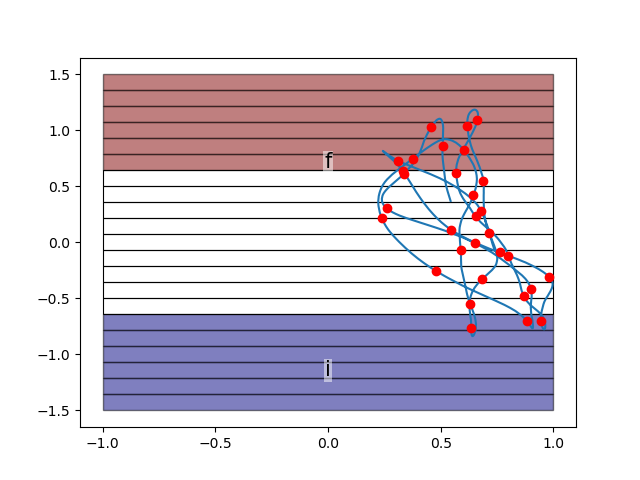
\includegraphics[width=0.9\linewidth]{simplenosl_1D}
	  	\label{simplenosl_1D}
  \end{minipage}
	\begin{minipage}[b]{0.5\textwidth}
  		\centering
  		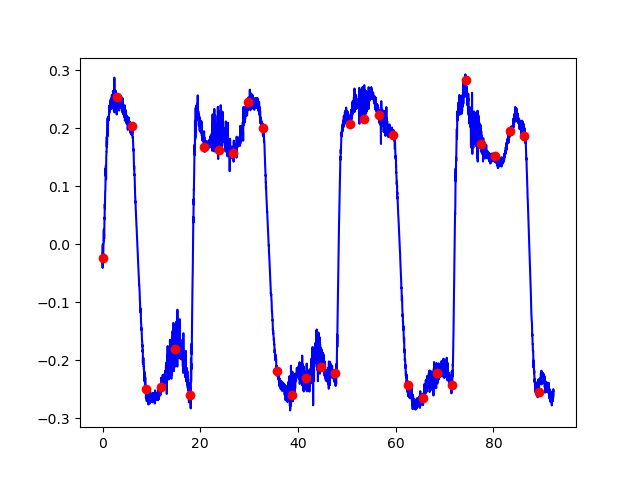
\includegraphics[width=0.9\linewidth]{simplenosl_1D_vel}
	  	\label{simplenosl_1D_vel}
  \end{minipage}
  \caption{Trajectory and velocity profile of the simple integrator model without self loops. The agent is trying to achieve 'go infinity often to i and f'.}
\end{figure}

\comment{Show the generated plans!}

This model is equivalent to the single integrator model.
We have been illustrating the advantages of self loops by doing one experiment with self loops and another experiment without self loops.
The FTS created without self loops needs to have a much finer discretization of the state space.
Whereas in the FTS with self loops the constraint on the minimal size of the state space discretization is only that the transient state on the velocity must counteract the effect of the noise.

\newcommand{\reg}[1]{\textit{reg #1}}
Other constraints apply on the sampling time: regions \reg{i} and \reg{f} needs to be reachable. If the sampling time is too high, the state might miss the target region.

When using a sampling time close to the transient time of the system, the reduction needs to take in account more states that belong to the transient states. This result in an increase of the modelled noise in the first integrator model.

\subsection{Comparison of the two results}
\begin{itemize}
\item compute the minimal number of states so that the model is usable (ie controllable)
\item compute the branching factor, the precision etc...
\item compute the amplitude of the noise in permanent state
\end{itemize}

Try to do it for different $\Delta n_u$, show that it does decrease the complexity for $\Delta n_u = 1$. Talk about the case $\Delta n_u = 0$ which correspond to the single integrator case (see part \ref{sec:single_int}).

Comparison to the double integrator case, show how the noise is evolving. Compare the size of the successors between the case where the discretization of the reduced state (velocity in this case) is lower than the steady state of the reduced state for a stable sequence. Basically, in one case, the size of the successors is growing (expansion of the successors) in the reduced approach, the size of the successors is reducing (but is bigger than the other one).


\comment{Try to show the 2 abstractions on top of each other to visualize what happened after the reduction}.

\paragraph{Sensitivity to noise}:
Please note that this model is less sensible to the noise on velocity as only the position is observed.
We have been noticing that this model was much easier to use thanks to this property.

\subsection{Experiments over 2 axes}

The previous study show the link between the precision and the complexity of the abstraction that we used.
In this part we will use the previous results in order to solve the following problem for different size of the environment:

\begin{figure}
	\center
	\includestandalone[width=0.5\textwidth]{2D_env_problem}
	\caption{Testing environment for the quadricopter.}
	\label{fig:environment}
\end{figure}

\comment{Show the simulation, the runs and so on.}


\subsection{Real case scenarios}

\begin{figure}[!ht]
  \centering
  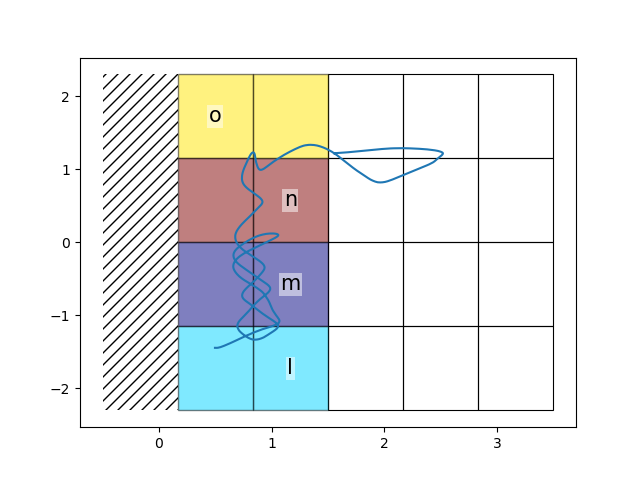
\includegraphics[width=0.9\linewidth]{real_case_scenarios}
  \caption{A trajectory in the state space $(x,v)$.}
\end{figure}

We have been using the first integrator model in this case (this is the more relevant in the scenario of the wind power).

\subsection{Discussion over the different models}
See table \ref{comparaison_table}.

\paragraph{Method:}
the comparison the different abstractions does not make any sense.
For example, in the second integrator abstraction, the discretization of the state space can be chosen to be the same than the reduced model, but we can always increase the precision over the velocity state.
We need to find a method that does not depend on a wrong parametrization of the method. Maybe defined the way we have been choosing the different abstraction (optimization criteria)?
So we need to use a standardized method in order to compare them.
For example, the minimum controllable abstraction might be a good choice.

There is no better abstraction, so we need to play with the parameters to show in which case the reduction is better than the original model.

